%!TEX root = nips2013.tex
\section{Learner Engagement in MOOCs}
\label{sec:learner_engage}

Since student responses are not directly observed in an online course, engagement cannot be easily determined, but rather it can be inferred by interpreting behavioral patterns which indicate student's level and type of involvement. 

In order to model learner engagement we first identify the relevant online behavioral activities of learners. These activities include several modes of interaction, for example passively watching lecture videos or actively answering quizzes during the lecture. Forum Activities include 1) \textit{Posting behavior} by the learner 2) \textit{Subscribing/viewing/voting} on content posted by others. Learners also demonstrate engagement by following course material such as video lectures, notes and take the assessments associated with them. Unlike a classroom setting where there is a schedule for a lecture/quiz/assignment, MOOCs have more leeway for completing course material and the assessments. Learners can be classified as on time, behind or not attempted based on when they complete the lectures, quizzes and assignments. 

Learners posting actively in the discussion forums can act as a good indicator of learner engagement, since forums are the only means of interaction in a MOOC setting.
Learners can use the forum posts to convey the satisfaction or dissatisfaction with course and possible provide indications of their interest in the class and motivation to complete it.
A finer analysis of the content of the posts is essential to conclude that the learner is engaged.
In order to use this information, in addition to the behavioral indicators above, we include linguistic indicators describing the posts content that could provide indication of the learner's engagement/disengagement. We use an automated tool (OpinionFinder, \cite{opinionfinder}) to annotate the form posts with two types of labels: subjectivity of content in posts and sentiment polarity of post content.

 Figure \ref{subj-disrtech} demonstrates the importance of capturing this information. The figure depicts the use of subjective expressions in forum content compared to the reaction these posts attract (measure in votes). The increasing trend of votes for presence of subjective expressions is indicative of the fact that posts containing subjective expressions invite more attention and trigger engagement.

Based on these two types of signals, we categorize learner engagement into the following types:

\textbf {Active Engagement.} Assigned to learners who show explicit signs of engagement by posting on the discussion forums, submitting quizzes and assessments. These signs require an active involvement from the learner.

\textbf{Passive Engagement.} Assigned to learners who show more implicit signs of engagement by viewing, subscribing or voting on posts/comments on discussion forums and views lectures. These users typically do not make an active effort to participate.

\textbf{Disengaged.} Learners that show signs of getting disengaged from the course, either by posting text that indicate their disengagement or show a significant decrease in posting, viewing, voting and assessment submitting activity.

%<example of a forum post that suggests disengagement.> \\
%<graph showing correlation between student participation in forums and course grades> \\
%<graphs showing correlation of subjectivity/polarity to performance>

\begin{figure} [ht]
\label{subj-disrtech}
\begin{center}
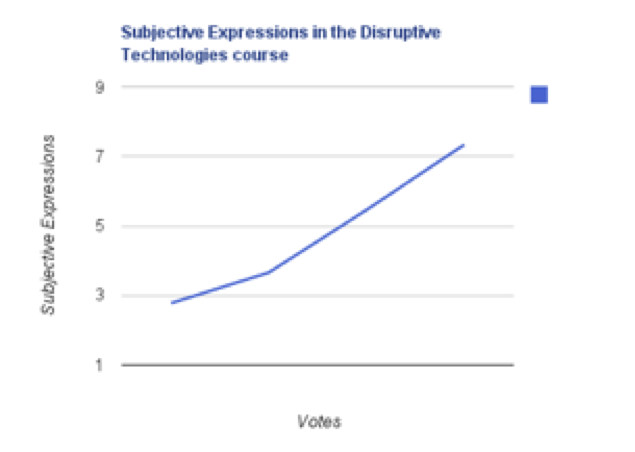
\includegraphics[width = 3.0in, height = 2in]{subjectivity-disrtech.png}
\caption{Subjectivity vs.\ votes.}
\end{center}
\end{figure}

We are interested in modeling engagement and reasoning about which form(s) of engagement are strong indicators of performance. 

